\documentclass[14pt]{extarticle}
\usepackage[letterpaper,top=20mm,bottom=20mm,left=16mm,right=16mm,headheight=16pt,headsep=7mm,footskip=10mm]{geometry}
\usepackage[T1]{fontenc}
\usepackage{tgheros}
\renewcommand{\familydefault}{\sfdefault}
\usepackage{tikz}
\usetikzlibrary{arrows.meta,decorations.pathreplacing}
\usepackage{fancyhdr}
\usepackage{xcolor}
\definecolor{cardred}{RGB}{206,38,38}
\definecolor{cardblue}{RGB}{28,92,196}
\colorlet{stripred}{cardred!32}
\colorlet{stripblue}{cardblue!28}
\colorlet{panelgrey}{black!20}
\colorlet{boxgrey}{black!45}
\tikzset{cardedge/.style={draw=black!70,line width=0.5pt}}
\pagestyle{fancy}
\fancyhf{}
\fancyhead[L]{\small Week 58 / Fair division / K--1}
\fancyfoot[L]{\small Bellingham Math Circle / Week 58 / W58-RV-K-v1}
\fancyfoot[R]{\small \thepage}
\renewcommand{\headrulewidth}{0.4pt}
\renewcommand{\footrulewidth}{0pt}
\setlength{\parindent}{0pt}
\setlength{\parskip}{4pt}
\newcommand{\prob}[1]{\par\noindent\textbf{Problem #1:} }
\begin{document}
A train is a row of goods cards. To share a train, pull it apart between cards and put each piece into one of two trays. A tray may get more than one piece. Both trays must get the same number of red cards and the same number of blue cards.
\begin{center}
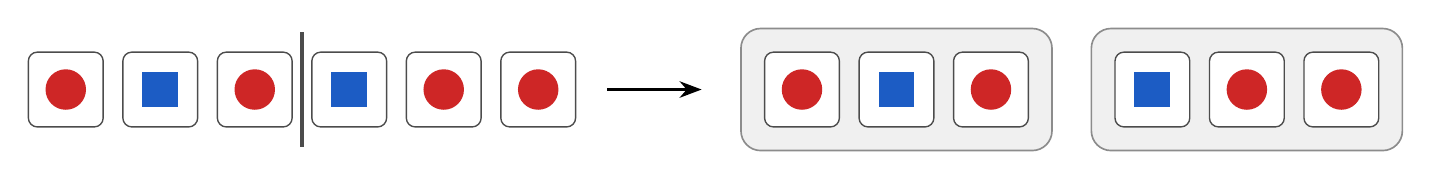
\begin{tikzpicture}[x=1mm,y=1mm]
\draw[cardedge, fill=white, rounded corners=1.14mm] (0,0) rectangle (9.5,9.5);
\fill[cardred] (4.75,4.75) circle (2.57mm);
\draw[cardedge, fill=white, rounded corners=1.14mm] (12,0) rectangle (21.5,9.5);
\fill[cardblue] (14.47,2.47) rectangle (19.03,7.03);
\draw[cardedge, fill=white, rounded corners=1.14mm] (24,0) rectangle (33.5,9.5);
\fill[cardred] (28.75,4.75) circle (2.57mm);
\draw[cardedge, fill=white, rounded corners=1.14mm] (36,0) rectangle (45.5,9.5);
\fill[cardblue] (38.47,2.47) rectangle (43.03,7.03);
\draw[cardedge, fill=white, rounded corners=1.14mm] (48,0) rectangle (57.5,9.5);
\fill[cardred] (52.75,4.75) circle (2.57mm);
\draw[cardedge, fill=white, rounded corners=1.14mm] (60,0) rectangle (69.5,9.5);
\fill[cardred] (64.75,4.75) circle (2.57mm);
\draw[black!70, line width=1.4pt] (34.75,-2.5) -- (34.75,12);
\draw[-{Stealth[length=2.8mm]}, line width=0.9pt] (73.5,4.75) -- (85.5,4.75);
\draw[black!45, fill=black!6, line width=0.6pt, rounded corners=2.5mm] (90.5,-3) rectangle (130,12.5);
\draw[cardedge, fill=white, rounded corners=1.14mm] (93.5,0) rectangle (103,9.5);
\fill[cardred] (98.25,4.75) circle (2.57mm);
\draw[cardedge, fill=white, rounded corners=1.14mm] (105.5,0) rectangle (115,9.5);
\fill[cardblue] (107.97,2.47) rectangle (112.53,7.03);
\draw[cardedge, fill=white, rounded corners=1.14mm] (117.5,0) rectangle (127,9.5);
\fill[cardred] (122.25,4.75) circle (2.57mm);
\draw[black!45, fill=black!6, line width=0.6pt, rounded corners=2.5mm] (135,-3) rectangle (174.5,12.5);
\draw[cardedge, fill=white, rounded corners=1.14mm] (138,0) rectangle (147.5,9.5);
\fill[cardblue] (140.47,2.47) rectangle (145.03,7.03);
\draw[cardedge, fill=white, rounded corners=1.14mm] (150,0) rectangle (159.5,9.5);
\fill[cardred] (154.75,4.75) circle (2.57mm);
\draw[cardedge, fill=white, rounded corners=1.14mm] (162,0) rectangle (171.5,9.5);
\fill[cardred] (166.75,4.75) circle (2.57mm);
\end{tikzpicture}
\end{center}
\vspace{1mm}
\prob{1}Make each train. Share it by pulling it apart at as few places as you can, and draw a line at each place.
\vspace{1mm}
\begin{center}
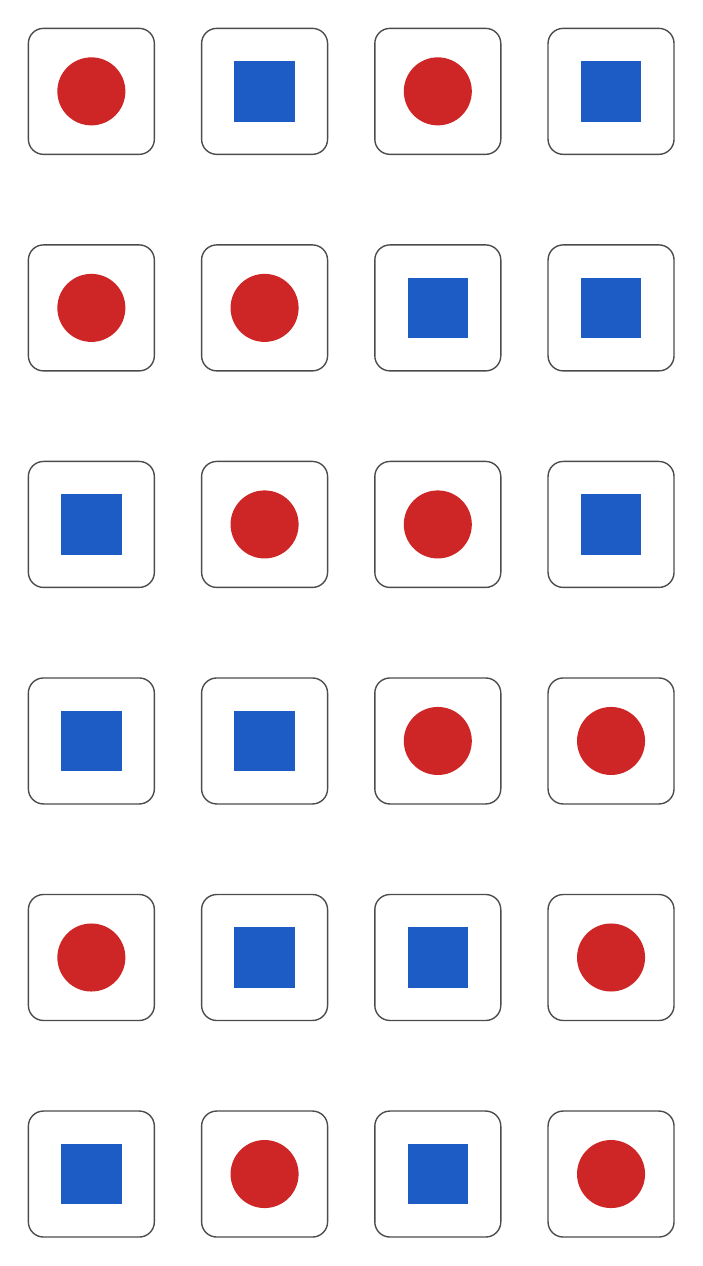
\begin{tikzpicture}[x=1mm,y=1mm]
\draw[cardedge, fill=white, rounded corners=1.92mm] (0,0) rectangle (16,16);
\fill[cardred] (8,8) circle (4.32mm);
\draw[cardedge, fill=white, rounded corners=1.92mm] (22,0) rectangle (38,16);
\fill[cardblue] (26.16,4.16) rectangle (33.84,11.84);
\draw[cardedge, fill=white, rounded corners=1.92mm] (44,0) rectangle (60,16);
\fill[cardred] (52,8) circle (4.32mm);
\draw[cardedge, fill=white, rounded corners=1.92mm] (66,0) rectangle (82,16);
\fill[cardblue] (70.16,4.16) rectangle (77.84,11.84);
\draw[cardedge, fill=white, rounded corners=1.92mm] (0,-27.5) rectangle (16,-11.5);
\fill[cardred] (8,-19.5) circle (4.32mm);
\draw[cardedge, fill=white, rounded corners=1.92mm] (22,-27.5) rectangle (38,-11.5);
\fill[cardred] (30,-19.5) circle (4.32mm);
\draw[cardedge, fill=white, rounded corners=1.92mm] (44,-27.5) rectangle (60,-11.5);
\fill[cardblue] (48.16,-23.34) rectangle (55.84,-15.66);
\draw[cardedge, fill=white, rounded corners=1.92mm] (66,-27.5) rectangle (82,-11.5);
\fill[cardblue] (70.16,-23.34) rectangle (77.84,-15.66);
\draw[cardedge, fill=white, rounded corners=1.92mm] (0,-55) rectangle (16,-39);
\fill[cardblue] (4.16,-50.84) rectangle (11.84,-43.16);
\draw[cardedge, fill=white, rounded corners=1.92mm] (22,-55) rectangle (38,-39);
\fill[cardred] (30,-47) circle (4.32mm);
\draw[cardedge, fill=white, rounded corners=1.92mm] (44,-55) rectangle (60,-39);
\fill[cardred] (52,-47) circle (4.32mm);
\draw[cardedge, fill=white, rounded corners=1.92mm] (66,-55) rectangle (82,-39);
\fill[cardblue] (70.16,-50.84) rectangle (77.84,-43.16);
\draw[cardedge, fill=white, rounded corners=1.92mm] (0,-82.5) rectangle (16,-66.5);
\fill[cardblue] (4.16,-78.34) rectangle (11.84,-70.66);
\draw[cardedge, fill=white, rounded corners=1.92mm] (22,-82.5) rectangle (38,-66.5);
\fill[cardblue] (26.16,-78.34) rectangle (33.84,-70.66);
\draw[cardedge, fill=white, rounded corners=1.92mm] (44,-82.5) rectangle (60,-66.5);
\fill[cardred] (52,-74.5) circle (4.32mm);
\draw[cardedge, fill=white, rounded corners=1.92mm] (66,-82.5) rectangle (82,-66.5);
\fill[cardred] (74,-74.5) circle (4.32mm);
\draw[cardedge, fill=white, rounded corners=1.92mm] (0,-110) rectangle (16,-94);
\fill[cardred] (8,-102) circle (4.32mm);
\draw[cardedge, fill=white, rounded corners=1.92mm] (22,-110) rectangle (38,-94);
\fill[cardblue] (26.16,-105.84) rectangle (33.84,-98.16);
\draw[cardedge, fill=white, rounded corners=1.92mm] (44,-110) rectangle (60,-94);
\fill[cardblue] (48.16,-105.84) rectangle (55.84,-98.16);
\draw[cardedge, fill=white, rounded corners=1.92mm] (66,-110) rectangle (82,-94);
\fill[cardred] (74,-102) circle (4.32mm);
\draw[cardedge, fill=white, rounded corners=1.92mm] (0,-137.5) rectangle (16,-121.5);
\fill[cardblue] (4.16,-133.34) rectangle (11.84,-125.66);
\draw[cardedge, fill=white, rounded corners=1.92mm] (22,-137.5) rectangle (38,-121.5);
\fill[cardred] (30,-129.5) circle (4.32mm);
\draw[cardedge, fill=white, rounded corners=1.92mm] (44,-137.5) rectangle (60,-121.5);
\fill[cardblue] (48.16,-133.34) rectangle (55.84,-125.66);
\draw[cardedge, fill=white, rounded corners=1.92mm] (66,-137.5) rectangle (82,-121.5);
\fill[cardred] (74,-129.5) circle (4.32mm);
\end{tikzpicture}
\end{center}
\newpage
\prob{2}Make each train and share it, pulling it apart at as few places as you can. Draw a line at each place, or cross out the train if it cannot be shared.
\vspace{4mm}
\begin{center}
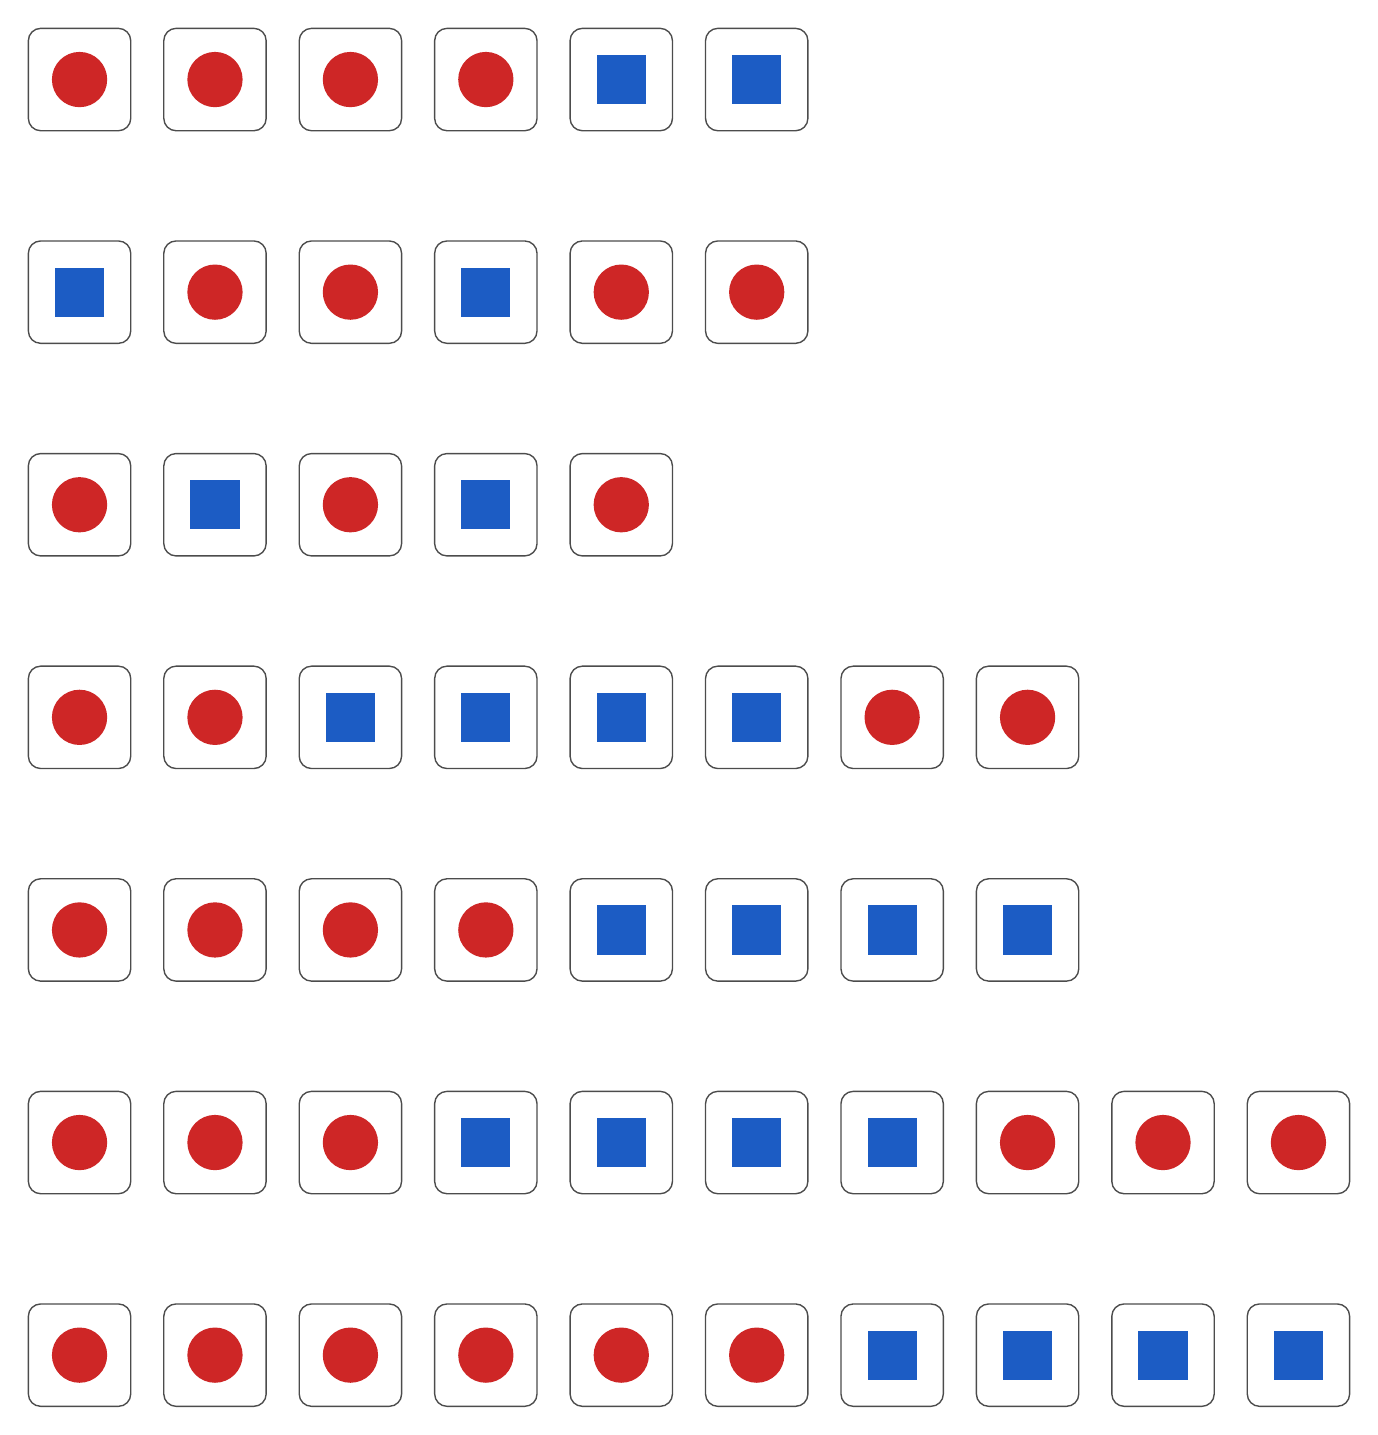
\begin{tikzpicture}[x=1mm,y=1mm]
\draw[cardedge, fill=white, rounded corners=1.56mm] (0,0) rectangle (13,13);
\fill[cardred] (6.5,6.5) circle (3.51mm);
\draw[cardedge, fill=white, rounded corners=1.56mm] (17.2,0) rectangle (30.2,13);
\fill[cardred] (23.7,6.5) circle (3.51mm);
\draw[cardedge, fill=white, rounded corners=1.56mm] (34.4,0) rectangle (47.4,13);
\fill[cardred] (40.9,6.5) circle (3.51mm);
\draw[cardedge, fill=white, rounded corners=1.56mm] (51.6,0) rectangle (64.6,13);
\fill[cardred] (58.1,6.5) circle (3.51mm);
\draw[cardedge, fill=white, rounded corners=1.56mm] (68.8,0) rectangle (81.8,13);
\fill[cardblue] (72.18,3.38) rectangle (78.42,9.62);
\draw[cardedge, fill=white, rounded corners=1.56mm] (86,0) rectangle (99,13);
\fill[cardblue] (89.38,3.38) rectangle (95.62,9.62);
\draw[cardedge, fill=white, rounded corners=1.56mm] (0,-27) rectangle (13,-14);
\fill[cardblue] (3.38,-23.62) rectangle (9.62,-17.38);
\draw[cardedge, fill=white, rounded corners=1.56mm] (17.2,-27) rectangle (30.2,-14);
\fill[cardred] (23.7,-20.5) circle (3.51mm);
\draw[cardedge, fill=white, rounded corners=1.56mm] (34.4,-27) rectangle (47.4,-14);
\fill[cardred] (40.9,-20.5) circle (3.51mm);
\draw[cardedge, fill=white, rounded corners=1.56mm] (51.6,-27) rectangle (64.6,-14);
\fill[cardblue] (54.98,-23.62) rectangle (61.22,-17.38);
\draw[cardedge, fill=white, rounded corners=1.56mm] (68.8,-27) rectangle (81.8,-14);
\fill[cardred] (75.3,-20.5) circle (3.51mm);
\draw[cardedge, fill=white, rounded corners=1.56mm] (86,-27) rectangle (99,-14);
\fill[cardred] (92.5,-20.5) circle (3.51mm);
\draw[cardedge, fill=white, rounded corners=1.56mm] (0,-54) rectangle (13,-41);
\fill[cardred] (6.5,-47.5) circle (3.51mm);
\draw[cardedge, fill=white, rounded corners=1.56mm] (17.2,-54) rectangle (30.2,-41);
\fill[cardblue] (20.58,-50.62) rectangle (26.82,-44.38);
\draw[cardedge, fill=white, rounded corners=1.56mm] (34.4,-54) rectangle (47.4,-41);
\fill[cardred] (40.9,-47.5) circle (3.51mm);
\draw[cardedge, fill=white, rounded corners=1.56mm] (51.6,-54) rectangle (64.6,-41);
\fill[cardblue] (54.98,-50.62) rectangle (61.22,-44.38);
\draw[cardedge, fill=white, rounded corners=1.56mm] (68.8,-54) rectangle (81.8,-41);
\fill[cardred] (75.3,-47.5) circle (3.51mm);
\draw[cardedge, fill=white, rounded corners=1.56mm] (0,-81) rectangle (13,-68);
\fill[cardred] (6.5,-74.5) circle (3.51mm);
\draw[cardedge, fill=white, rounded corners=1.56mm] (17.2,-81) rectangle (30.2,-68);
\fill[cardred] (23.7,-74.5) circle (3.51mm);
\draw[cardedge, fill=white, rounded corners=1.56mm] (34.4,-81) rectangle (47.4,-68);
\fill[cardblue] (37.78,-77.62) rectangle (44.02,-71.38);
\draw[cardedge, fill=white, rounded corners=1.56mm] (51.6,-81) rectangle (64.6,-68);
\fill[cardblue] (54.98,-77.62) rectangle (61.22,-71.38);
\draw[cardedge, fill=white, rounded corners=1.56mm] (68.8,-81) rectangle (81.8,-68);
\fill[cardblue] (72.18,-77.62) rectangle (78.42,-71.38);
\draw[cardedge, fill=white, rounded corners=1.56mm] (86,-81) rectangle (99,-68);
\fill[cardblue] (89.38,-77.62) rectangle (95.62,-71.38);
\draw[cardedge, fill=white, rounded corners=1.56mm] (103.2,-81) rectangle (116.2,-68);
\fill[cardred] (109.7,-74.5) circle (3.51mm);
\draw[cardedge, fill=white, rounded corners=1.56mm] (120.4,-81) rectangle (133.4,-68);
\fill[cardred] (126.9,-74.5) circle (3.51mm);
\draw[cardedge, fill=white, rounded corners=1.56mm] (0,-108) rectangle (13,-95);
\fill[cardred] (6.5,-101.5) circle (3.51mm);
\draw[cardedge, fill=white, rounded corners=1.56mm] (17.2,-108) rectangle (30.2,-95);
\fill[cardred] (23.7,-101.5) circle (3.51mm);
\draw[cardedge, fill=white, rounded corners=1.56mm] (34.4,-108) rectangle (47.4,-95);
\fill[cardred] (40.9,-101.5) circle (3.51mm);
\draw[cardedge, fill=white, rounded corners=1.56mm] (51.6,-108) rectangle (64.6,-95);
\fill[cardred] (58.1,-101.5) circle (3.51mm);
\draw[cardedge, fill=white, rounded corners=1.56mm] (68.8,-108) rectangle (81.8,-95);
\fill[cardblue] (72.18,-104.62) rectangle (78.42,-98.38);
\draw[cardedge, fill=white, rounded corners=1.56mm] (86,-108) rectangle (99,-95);
\fill[cardblue] (89.38,-104.62) rectangle (95.62,-98.38);
\draw[cardedge, fill=white, rounded corners=1.56mm] (103.2,-108) rectangle (116.2,-95);
\fill[cardblue] (106.58,-104.62) rectangle (112.82,-98.38);
\draw[cardedge, fill=white, rounded corners=1.56mm] (120.4,-108) rectangle (133.4,-95);
\fill[cardblue] (123.78,-104.62) rectangle (130.02,-98.38);
\draw[cardedge, fill=white, rounded corners=1.56mm] (0,-135) rectangle (13,-122);
\fill[cardred] (6.5,-128.5) circle (3.51mm);
\draw[cardedge, fill=white, rounded corners=1.56mm] (17.2,-135) rectangle (30.2,-122);
\fill[cardred] (23.7,-128.5) circle (3.51mm);
\draw[cardedge, fill=white, rounded corners=1.56mm] (34.4,-135) rectangle (47.4,-122);
\fill[cardred] (40.9,-128.5) circle (3.51mm);
\draw[cardedge, fill=white, rounded corners=1.56mm] (51.6,-135) rectangle (64.6,-122);
\fill[cardblue] (54.98,-131.62) rectangle (61.22,-125.38);
\draw[cardedge, fill=white, rounded corners=1.56mm] (68.8,-135) rectangle (81.8,-122);
\fill[cardblue] (72.18,-131.62) rectangle (78.42,-125.38);
\draw[cardedge, fill=white, rounded corners=1.56mm] (86,-135) rectangle (99,-122);
\fill[cardblue] (89.38,-131.62) rectangle (95.62,-125.38);
\draw[cardedge, fill=white, rounded corners=1.56mm] (103.2,-135) rectangle (116.2,-122);
\fill[cardblue] (106.58,-131.62) rectangle (112.82,-125.38);
\draw[cardedge, fill=white, rounded corners=1.56mm] (120.4,-135) rectangle (133.4,-122);
\fill[cardred] (126.9,-128.5) circle (3.51mm);
\draw[cardedge, fill=white, rounded corners=1.56mm] (137.6,-135) rectangle (150.6,-122);
\fill[cardred] (144.1,-128.5) circle (3.51mm);
\draw[cardedge, fill=white, rounded corners=1.56mm] (154.8,-135) rectangle (167.8,-122);
\fill[cardred] (161.3,-128.5) circle (3.51mm);
\draw[cardedge, fill=white, rounded corners=1.56mm] (0,-162) rectangle (13,-149);
\fill[cardred] (6.5,-155.5) circle (3.51mm);
\draw[cardedge, fill=white, rounded corners=1.56mm] (17.2,-162) rectangle (30.2,-149);
\fill[cardred] (23.7,-155.5) circle (3.51mm);
\draw[cardedge, fill=white, rounded corners=1.56mm] (34.4,-162) rectangle (47.4,-149);
\fill[cardred] (40.9,-155.5) circle (3.51mm);
\draw[cardedge, fill=white, rounded corners=1.56mm] (51.6,-162) rectangle (64.6,-149);
\fill[cardred] (58.1,-155.5) circle (3.51mm);
\draw[cardedge, fill=white, rounded corners=1.56mm] (68.8,-162) rectangle (81.8,-149);
\fill[cardred] (75.3,-155.5) circle (3.51mm);
\draw[cardedge, fill=white, rounded corners=1.56mm] (86,-162) rectangle (99,-149);
\fill[cardred] (92.5,-155.5) circle (3.51mm);
\draw[cardedge, fill=white, rounded corners=1.56mm] (103.2,-162) rectangle (116.2,-149);
\fill[cardblue] (106.58,-158.62) rectangle (112.82,-152.38);
\draw[cardedge, fill=white, rounded corners=1.56mm] (120.4,-162) rectangle (133.4,-149);
\fill[cardblue] (123.78,-158.62) rectangle (130.02,-152.38);
\draw[cardedge, fill=white, rounded corners=1.56mm] (137.6,-162) rectangle (150.6,-149);
\fill[cardblue] (140.98,-158.62) rectangle (147.22,-152.38);
\draw[cardedge, fill=white, rounded corners=1.56mm] (154.8,-162) rectangle (167.8,-149);
\fill[cardblue] (158.18,-158.62) rectangle (164.42,-152.38);
\path (0,0) -- (167.8,0);
\end{tikzpicture}
\end{center}
\newpage
\prob{3}One player makes a train with four red cards and four blue cards that cannot be shared by pulling it apart at only one place. The other player tries to share it that way. Draw each train that could not be shared.
\vspace{4mm}
\begin{center}

\begin{tikzpicture}[x=1mm,y=1mm]
\draw[boxgrey, line width=0.5pt, rounded corners=1.56mm] (0,0) rectangle (13,13);
\draw[boxgrey, line width=0.5pt, rounded corners=1.56mm] (17.2,0) rectangle (30.2,13);
\draw[boxgrey, line width=0.5pt, rounded corners=1.56mm] (34.4,0) rectangle (47.4,13);
\draw[boxgrey, line width=0.5pt, rounded corners=1.56mm] (51.6,0) rectangle (64.6,13);
\draw[boxgrey, line width=0.5pt, rounded corners=1.56mm] (68.8,0) rectangle (81.8,13);
\draw[boxgrey, line width=0.5pt, rounded corners=1.56mm] (86,0) rectangle (99,13);
\draw[boxgrey, line width=0.5pt, rounded corners=1.56mm] (103.2,0) rectangle (116.2,13);
\draw[boxgrey, line width=0.5pt, rounded corners=1.56mm] (120.4,0) rectangle (133.4,13);
\draw[boxgrey, line width=0.5pt, rounded corners=1.56mm] (0,-27) rectangle (13,-14);
\draw[boxgrey, line width=0.5pt, rounded corners=1.56mm] (17.2,-27) rectangle (30.2,-14);
\draw[boxgrey, line width=0.5pt, rounded corners=1.56mm] (34.4,-27) rectangle (47.4,-14);
\draw[boxgrey, line width=0.5pt, rounded corners=1.56mm] (51.6,-27) rectangle (64.6,-14);
\draw[boxgrey, line width=0.5pt, rounded corners=1.56mm] (68.8,-27) rectangle (81.8,-14);
\draw[boxgrey, line width=0.5pt, rounded corners=1.56mm] (86,-27) rectangle (99,-14);
\draw[boxgrey, line width=0.5pt, rounded corners=1.56mm] (103.2,-27) rectangle (116.2,-14);
\draw[boxgrey, line width=0.5pt, rounded corners=1.56mm] (120.4,-27) rectangle (133.4,-14);
\draw[boxgrey, line width=0.5pt, rounded corners=1.56mm] (0,-54) rectangle (13,-41);
\draw[boxgrey, line width=0.5pt, rounded corners=1.56mm] (17.2,-54) rectangle (30.2,-41);
\draw[boxgrey, line width=0.5pt, rounded corners=1.56mm] (34.4,-54) rectangle (47.4,-41);
\draw[boxgrey, line width=0.5pt, rounded corners=1.56mm] (51.6,-54) rectangle (64.6,-41);
\draw[boxgrey, line width=0.5pt, rounded corners=1.56mm] (68.8,-54) rectangle (81.8,-41);
\draw[boxgrey, line width=0.5pt, rounded corners=1.56mm] (86,-54) rectangle (99,-41);
\draw[boxgrey, line width=0.5pt, rounded corners=1.56mm] (103.2,-54) rectangle (116.2,-41);
\draw[boxgrey, line width=0.5pt, rounded corners=1.56mm] (120.4,-54) rectangle (133.4,-41);
\draw[boxgrey, line width=0.5pt, rounded corners=1.56mm] (0,-81) rectangle (13,-68);
\draw[boxgrey, line width=0.5pt, rounded corners=1.56mm] (17.2,-81) rectangle (30.2,-68);
\draw[boxgrey, line width=0.5pt, rounded corners=1.56mm] (34.4,-81) rectangle (47.4,-68);
\draw[boxgrey, line width=0.5pt, rounded corners=1.56mm] (51.6,-81) rectangle (64.6,-68);
\draw[boxgrey, line width=0.5pt, rounded corners=1.56mm] (68.8,-81) rectangle (81.8,-68);
\draw[boxgrey, line width=0.5pt, rounded corners=1.56mm] (86,-81) rectangle (99,-68);
\draw[boxgrey, line width=0.5pt, rounded corners=1.56mm] (103.2,-81) rectangle (116.2,-68);
\draw[boxgrey, line width=0.5pt, rounded corners=1.56mm] (120.4,-81) rectangle (133.4,-68);
\draw[boxgrey, line width=0.5pt, rounded corners=1.56mm] (0,-108) rectangle (13,-95);
\draw[boxgrey, line width=0.5pt, rounded corners=1.56mm] (17.2,-108) rectangle (30.2,-95);
\draw[boxgrey, line width=0.5pt, rounded corners=1.56mm] (34.4,-108) rectangle (47.4,-95);
\draw[boxgrey, line width=0.5pt, rounded corners=1.56mm] (51.6,-108) rectangle (64.6,-95);
\draw[boxgrey, line width=0.5pt, rounded corners=1.56mm] (68.8,-108) rectangle (81.8,-95);
\draw[boxgrey, line width=0.5pt, rounded corners=1.56mm] (86,-108) rectangle (99,-95);
\draw[boxgrey, line width=0.5pt, rounded corners=1.56mm] (103.2,-108) rectangle (116.2,-95);
\draw[boxgrey, line width=0.5pt, rounded corners=1.56mm] (120.4,-108) rectangle (133.4,-95);
\draw[boxgrey, line width=0.5pt, rounded corners=1.56mm] (0,-135) rectangle (13,-122);
\draw[boxgrey, line width=0.5pt, rounded corners=1.56mm] (17.2,-135) rectangle (30.2,-122);
\draw[boxgrey, line width=0.5pt, rounded corners=1.56mm] (34.4,-135) rectangle (47.4,-122);
\draw[boxgrey, line width=0.5pt, rounded corners=1.56mm] (51.6,-135) rectangle (64.6,-122);
\draw[boxgrey, line width=0.5pt, rounded corners=1.56mm] (68.8,-135) rectangle (81.8,-122);
\draw[boxgrey, line width=0.5pt, rounded corners=1.56mm] (86,-135) rectangle (99,-122);
\draw[boxgrey, line width=0.5pt, rounded corners=1.56mm] (103.2,-135) rectangle (116.2,-122);
\draw[boxgrey, line width=0.5pt, rounded corners=1.56mm] (120.4,-135) rectangle (133.4,-122);
\draw[boxgrey, line width=0.5pt, rounded corners=1.56mm] (0,-162) rectangle (13,-149);
\draw[boxgrey, line width=0.5pt, rounded corners=1.56mm] (17.2,-162) rectangle (30.2,-149);
\draw[boxgrey, line width=0.5pt, rounded corners=1.56mm] (34.4,-162) rectangle (47.4,-149);
\draw[boxgrey, line width=0.5pt, rounded corners=1.56mm] (51.6,-162) rectangle (64.6,-149);
\draw[boxgrey, line width=0.5pt, rounded corners=1.56mm] (68.8,-162) rectangle (81.8,-149);
\draw[boxgrey, line width=0.5pt, rounded corners=1.56mm] (86,-162) rectangle (99,-149);
\draw[boxgrey, line width=0.5pt, rounded corners=1.56mm] (103.2,-162) rectangle (116.2,-149);
\draw[boxgrey, line width=0.5pt, rounded corners=1.56mm] (120.4,-162) rectangle (133.4,-149);
\end{tikzpicture}
\end{center}
\newpage
\prob{4}Share one red and blue strip between the two trays so that both trays get the same amount of red and the same amount of blue. Mark where an adult should cut straight across the strip, using as few cuts as you can.
\vspace{8mm}
\begin{center}
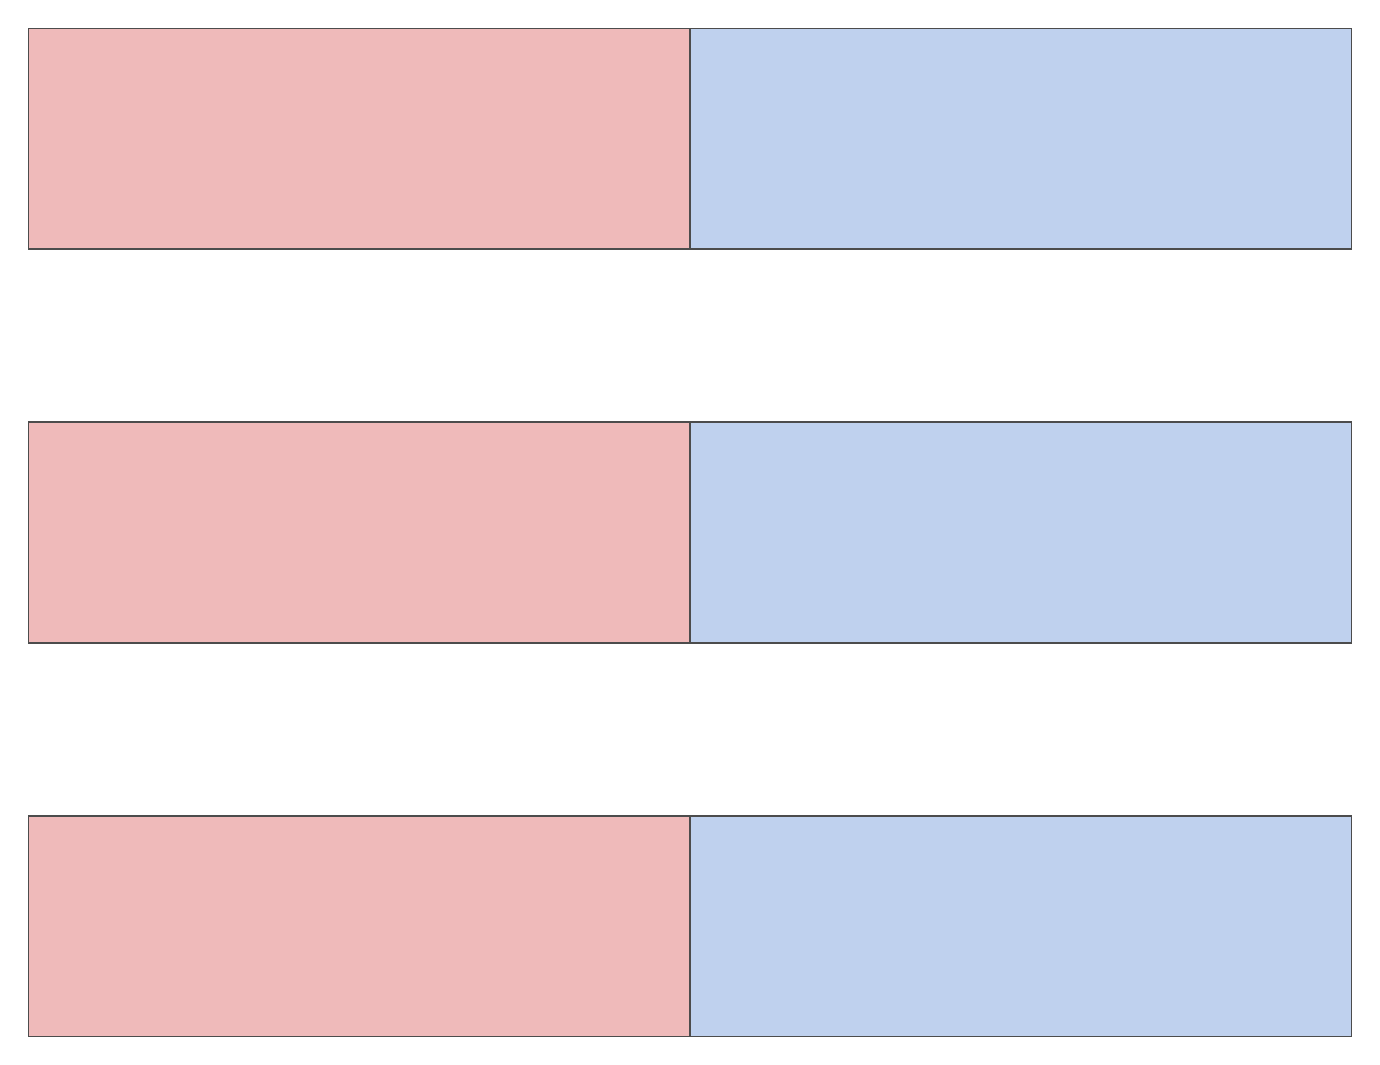
\begin{tikzpicture}[x=1mm,y=1mm]
\fill[stripred] (0,0) rectangle (84,28);
\fill[stripblue] (84,0) rectangle (168,28);
\draw[black!70, line width=0.6pt] (0,0) rectangle (168,28);
\draw[black!70, line width=0.6pt] (84,0) -- (84,28);
\fill[stripred] (0,-50) rectangle (84,-22);
\fill[stripblue] (84,-50) rectangle (168,-22);
\draw[black!70, line width=0.6pt] (0,-50) rectangle (168,-22);
\draw[black!70, line width=0.6pt] (84,-50) -- (84,-22);
\fill[stripred] (0,-100) rectangle (84,-72);
\fill[stripblue] (84,-100) rectangle (168,-72);
\draw[black!70, line width=0.6pt] (0,-100) rectangle (168,-72);
\draw[black!70, line width=0.6pt] (84,-100) -- (84,-72);
\end{tikzpicture}
\end{center}
\newpage
\prob{5}Can you make a train that has to be pulled apart at three places to share it? You may use up to six red cards and four blue cards.
\vspace{4mm}
\begin{center}
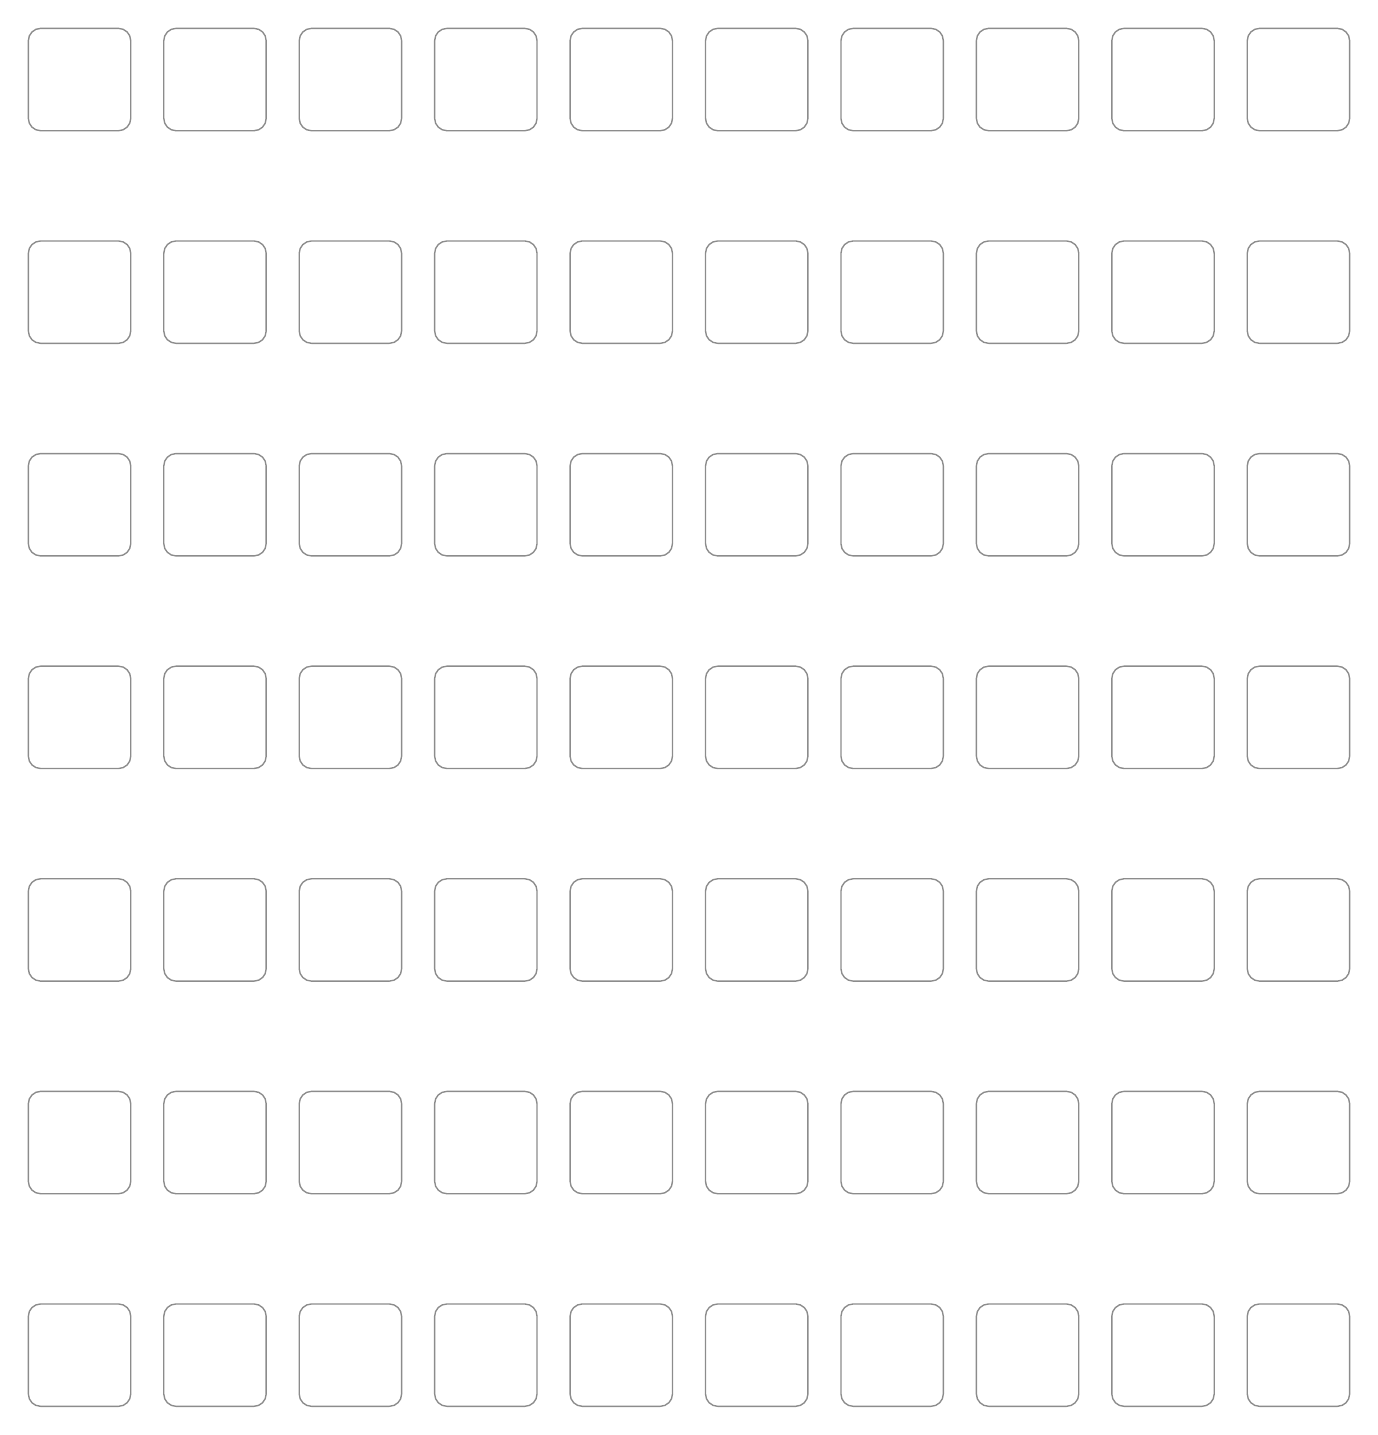
\begin{tikzpicture}[x=1mm,y=1mm]
\draw[boxgrey, line width=0.5pt, rounded corners=1.56mm] (0,0) rectangle (13,13);
\draw[boxgrey, line width=0.5pt, rounded corners=1.56mm] (17.2,0) rectangle (30.2,13);
\draw[boxgrey, line width=0.5pt, rounded corners=1.56mm] (34.4,0) rectangle (47.4,13);
\draw[boxgrey, line width=0.5pt, rounded corners=1.56mm] (51.6,0) rectangle (64.6,13);
\draw[boxgrey, line width=0.5pt, rounded corners=1.56mm] (68.8,0) rectangle (81.8,13);
\draw[boxgrey, line width=0.5pt, rounded corners=1.56mm] (86,0) rectangle (99,13);
\draw[boxgrey, line width=0.5pt, rounded corners=1.56mm] (103.2,0) rectangle (116.2,13);
\draw[boxgrey, line width=0.5pt, rounded corners=1.56mm] (120.4,0) rectangle (133.4,13);
\draw[boxgrey, line width=0.5pt, rounded corners=1.56mm] (137.6,0) rectangle (150.6,13);
\draw[boxgrey, line width=0.5pt, rounded corners=1.56mm] (154.8,0) rectangle (167.8,13);
\draw[boxgrey, line width=0.5pt, rounded corners=1.56mm] (0,-27) rectangle (13,-14);
\draw[boxgrey, line width=0.5pt, rounded corners=1.56mm] (17.2,-27) rectangle (30.2,-14);
\draw[boxgrey, line width=0.5pt, rounded corners=1.56mm] (34.4,-27) rectangle (47.4,-14);
\draw[boxgrey, line width=0.5pt, rounded corners=1.56mm] (51.6,-27) rectangle (64.6,-14);
\draw[boxgrey, line width=0.5pt, rounded corners=1.56mm] (68.8,-27) rectangle (81.8,-14);
\draw[boxgrey, line width=0.5pt, rounded corners=1.56mm] (86,-27) rectangle (99,-14);
\draw[boxgrey, line width=0.5pt, rounded corners=1.56mm] (103.2,-27) rectangle (116.2,-14);
\draw[boxgrey, line width=0.5pt, rounded corners=1.56mm] (120.4,-27) rectangle (133.4,-14);
\draw[boxgrey, line width=0.5pt, rounded corners=1.56mm] (137.6,-27) rectangle (150.6,-14);
\draw[boxgrey, line width=0.5pt, rounded corners=1.56mm] (154.8,-27) rectangle (167.8,-14);
\draw[boxgrey, line width=0.5pt, rounded corners=1.56mm] (0,-54) rectangle (13,-41);
\draw[boxgrey, line width=0.5pt, rounded corners=1.56mm] (17.2,-54) rectangle (30.2,-41);
\draw[boxgrey, line width=0.5pt, rounded corners=1.56mm] (34.4,-54) rectangle (47.4,-41);
\draw[boxgrey, line width=0.5pt, rounded corners=1.56mm] (51.6,-54) rectangle (64.6,-41);
\draw[boxgrey, line width=0.5pt, rounded corners=1.56mm] (68.8,-54) rectangle (81.8,-41);
\draw[boxgrey, line width=0.5pt, rounded corners=1.56mm] (86,-54) rectangle (99,-41);
\draw[boxgrey, line width=0.5pt, rounded corners=1.56mm] (103.2,-54) rectangle (116.2,-41);
\draw[boxgrey, line width=0.5pt, rounded corners=1.56mm] (120.4,-54) rectangle (133.4,-41);
\draw[boxgrey, line width=0.5pt, rounded corners=1.56mm] (137.6,-54) rectangle (150.6,-41);
\draw[boxgrey, line width=0.5pt, rounded corners=1.56mm] (154.8,-54) rectangle (167.8,-41);
\draw[boxgrey, line width=0.5pt, rounded corners=1.56mm] (0,-81) rectangle (13,-68);
\draw[boxgrey, line width=0.5pt, rounded corners=1.56mm] (17.2,-81) rectangle (30.2,-68);
\draw[boxgrey, line width=0.5pt, rounded corners=1.56mm] (34.4,-81) rectangle (47.4,-68);
\draw[boxgrey, line width=0.5pt, rounded corners=1.56mm] (51.6,-81) rectangle (64.6,-68);
\draw[boxgrey, line width=0.5pt, rounded corners=1.56mm] (68.8,-81) rectangle (81.8,-68);
\draw[boxgrey, line width=0.5pt, rounded corners=1.56mm] (86,-81) rectangle (99,-68);
\draw[boxgrey, line width=0.5pt, rounded corners=1.56mm] (103.2,-81) rectangle (116.2,-68);
\draw[boxgrey, line width=0.5pt, rounded corners=1.56mm] (120.4,-81) rectangle (133.4,-68);
\draw[boxgrey, line width=0.5pt, rounded corners=1.56mm] (137.6,-81) rectangle (150.6,-68);
\draw[boxgrey, line width=0.5pt, rounded corners=1.56mm] (154.8,-81) rectangle (167.8,-68);
\draw[boxgrey, line width=0.5pt, rounded corners=1.56mm] (0,-108) rectangle (13,-95);
\draw[boxgrey, line width=0.5pt, rounded corners=1.56mm] (17.2,-108) rectangle (30.2,-95);
\draw[boxgrey, line width=0.5pt, rounded corners=1.56mm] (34.4,-108) rectangle (47.4,-95);
\draw[boxgrey, line width=0.5pt, rounded corners=1.56mm] (51.6,-108) rectangle (64.6,-95);
\draw[boxgrey, line width=0.5pt, rounded corners=1.56mm] (68.8,-108) rectangle (81.8,-95);
\draw[boxgrey, line width=0.5pt, rounded corners=1.56mm] (86,-108) rectangle (99,-95);
\draw[boxgrey, line width=0.5pt, rounded corners=1.56mm] (103.2,-108) rectangle (116.2,-95);
\draw[boxgrey, line width=0.5pt, rounded corners=1.56mm] (120.4,-108) rectangle (133.4,-95);
\draw[boxgrey, line width=0.5pt, rounded corners=1.56mm] (137.6,-108) rectangle (150.6,-95);
\draw[boxgrey, line width=0.5pt, rounded corners=1.56mm] (154.8,-108) rectangle (167.8,-95);
\draw[boxgrey, line width=0.5pt, rounded corners=1.56mm] (0,-135) rectangle (13,-122);
\draw[boxgrey, line width=0.5pt, rounded corners=1.56mm] (17.2,-135) rectangle (30.2,-122);
\draw[boxgrey, line width=0.5pt, rounded corners=1.56mm] (34.4,-135) rectangle (47.4,-122);
\draw[boxgrey, line width=0.5pt, rounded corners=1.56mm] (51.6,-135) rectangle (64.6,-122);
\draw[boxgrey, line width=0.5pt, rounded corners=1.56mm] (68.8,-135) rectangle (81.8,-122);
\draw[boxgrey, line width=0.5pt, rounded corners=1.56mm] (86,-135) rectangle (99,-122);
\draw[boxgrey, line width=0.5pt, rounded corners=1.56mm] (103.2,-135) rectangle (116.2,-122);
\draw[boxgrey, line width=0.5pt, rounded corners=1.56mm] (120.4,-135) rectangle (133.4,-122);
\draw[boxgrey, line width=0.5pt, rounded corners=1.56mm] (137.6,-135) rectangle (150.6,-122);
\draw[boxgrey, line width=0.5pt, rounded corners=1.56mm] (154.8,-135) rectangle (167.8,-122);
\draw[boxgrey, line width=0.5pt, rounded corners=1.56mm] (0,-162) rectangle (13,-149);
\draw[boxgrey, line width=0.5pt, rounded corners=1.56mm] (17.2,-162) rectangle (30.2,-149);
\draw[boxgrey, line width=0.5pt, rounded corners=1.56mm] (34.4,-162) rectangle (47.4,-149);
\draw[boxgrey, line width=0.5pt, rounded corners=1.56mm] (51.6,-162) rectangle (64.6,-149);
\draw[boxgrey, line width=0.5pt, rounded corners=1.56mm] (68.8,-162) rectangle (81.8,-149);
\draw[boxgrey, line width=0.5pt, rounded corners=1.56mm] (86,-162) rectangle (99,-149);
\draw[boxgrey, line width=0.5pt, rounded corners=1.56mm] (103.2,-162) rectangle (116.2,-149);
\draw[boxgrey, line width=0.5pt, rounded corners=1.56mm] (120.4,-162) rectangle (133.4,-149);
\draw[boxgrey, line width=0.5pt, rounded corners=1.56mm] (137.6,-162) rectangle (150.6,-149);
\draw[boxgrey, line width=0.5pt, rounded corners=1.56mm] (154.8,-162) rectangle (167.8,-149);
\end{tikzpicture}
\end{center}

\end{document}
